\documentclass{ieeeaccess}

% --------------------------------------------
% Preamble
% --------------------------------------------
\usepackage{cite}
\usepackage{amsmath,amssymb,amsfonts}
\usepackage{algorithmic}
\usepackage{graphicx}
\usepackage{textcomp}

% Additional packages
\usepackage[english]{babel}
\usepackage[margins]{trackchanges}

\usepackage{xcolor}
\usepackage{soul}

% --------------------------------------------

\def\BibTeX{{\rm B\kern-.05em{\sc i\kern-.025em b}\kern-.08em
    T\kern-.1667em\lower.7ex\hbox{E}\kern-.125emX}}

% --------------------------------------------
% To print bibliography in order of citation:
\bibliographystyle{unsrt}		% Style of bibliography presentation
% \bibliographystyle{ieeetr}
% --------------------------------------------

\addeditor{JF}

\usepackage{array}
\newcolumntype{L}[1]{>{\raggedright\let\newline\\\arraybackslash\hspace{0pt}}m{#1}}
\newcolumntype{C}[1]{>{\centering\let\newline\\\arraybackslash\hspace{0pt}}m{#1}}
\newcolumntype{R}[1]{>{\raggedleft\let\newline\\\arraybackslash\hspace{0pt}}m{#1}}

\begin{document}

% header on first page
\history{Date of publication xxxx 00, 0000, date of current version xxxx 00, 0000.}
\doi{10.1109/ACCESS.2017.DOI}

\title{Simulation and Classification of Spatial Disorientation in a Flight use-case using Vestibular Stimulation}
\author{\uppercase{Jamilah Foucher}\authorrefmark{1}, \IEEEmembership{Member, IEEE},
\uppercase{Anne-Claire Collet}\authorrefmark{5}, \uppercase{Kevin Le Goff}\authorrefmark{3}, \uppercase{Thomas Rakotomamonjy}\authorrefmark{2}, \uppercase{Valerie Juppet}\authorrefmark{4}, \uppercase{Thomas Descatoire}\authorrefmark{4}, \uppercase{Jerémie Landrieu}\authorrefmark{1}, \uppercase{Marielle Plat-Robain}\authorrefmark{3}, \uppercase{François Denquin}\authorrefmark{1,2}, \uppercase{Arthur Grunwald}\authorrefmark{6}, \uppercase{Jean-Christophe Sarrazin}\authorrefmark{2}, and \uppercase{Benoît G. Bardy}.\authorrefmark{1}}
\address[1]{EuroMov Digital Health in Motion, Univ Montpellier and IMT Mines Ales, Montpellier 34090 France (e-mail: benoit.bardy@umontpellier.fr)}
\address[2]{DTIS, ONERA, Salon de Provence 13300 France}
\address[3]{AIRBUS, Toulouse 31000 France}
\address[4]{AIRBUS Helicopters, Marignane 13700 France}
\address[5]{Human Design Group, Toulouse 31000 France}
\address[6]{Technion, Israel Institute of Technology 32000 Israel}
\tfootnote{This project was supported by the French Department of Civil Aviation (DGAC) and by the European Union (FEDER iMOSE).}

\markboth
{Jamilah Foucher \headeretal: Preparation of Papers for IEEE TRANSACTIONS and JOURNALS}
{Benoît G. Bardy \headeretal: Preparation of Papers for IEEE TRANSACTIONS and JOURNALS}

\corresp{Corresponding authors: Jamilah Foucher (e-mail: j622amilah@gmail.com).}.

\begin{abstract}
\hl{A commonly used definition of spatial disorientation (SD) in aeronautics} is "an erroneous sense of one’s position and motion relative to the plane of the earth’s surface". SD has a wide range of situations and factors, but mainly it has been studied using reduced experimental contexts such as motion detection experimentation in isolation. Because there are many SD use-cases that are studied in isolation in a reduced manner, it is difficult to develop a generalized and fundamental understanding of the occurrence of SD and viable solutions. \hl{To investigate SD in a generalized manner, a two-part Human Activity Recognition (HAR) study consisting of an in-flight piloting use-case experiment and deep learning (DL) model prediction was performed.} The first part of the study was the creation of a generalized SD perception dataset using whole-body experimental motion detection methods in a naturalistic flight context; participant perceptual joystick response was measured during rotational or translational vestibular stimulation. \hl{The second part of the study consisted of HAR SD feature and model comparison. Human movement science domain knowledge for joystick response derived feature selection was exploited, and time and/or frequency signal contributions for sequential and spatial model architectures are investigated. Human behavior was interpreted from DL model parameters. A potential HAR SD feature was investigated using statistical analysis, comparing measurement trends of physical disorientation with respect to the motion detection label; the simulator sickness questionnaire (SSQ) disorientation sub-scale was used to quantify physical disorientation. The perceptual SD dataset was statistically proven to be representative of human motion detection behavior, demonstrating that the simulation environment was sufficient to generate a fidel SD context. DL modeling comparison analysis demonstrated that SD can be accurately predicted. Feature quantity, model type, models from use-case data, feature type, and label type significantly influenced prediction accuracy.} Finally, no significant relationship between physical disorientation and motion detection was found, indicating that two-sample before and after SSQ questionnaire-based methods are insufficient to uncover correlations with perceptual disorientation; a more frequent physical disorientation measure is needed.
\end{abstract}

\begin{keywords}
Aircraft navigation, human computer interaction, joystick perceptual response, machine learning algorithms, motion detection, spatial disorientation, vestibular dead reckoning, human activity recognition.
\end{keywords}

% \titlepgskip=-15pt

\maketitle

\section{INTRODUCTION}
% -------------------
% Description of SD
% -------------------
% - Define SD
% - State the problems of SD
%   1) SD happens often and result in serious accidents
%   2) it is difficult to recover from SD, the pilot must be able to think clearly and quickly when disorientation occurs
%   3) Current measures used in SD are questionnaires
%   4) Current solutions to treat SD
% - What exactly needs to be solved regarding SD
% - Last sentence : needs to talk about SD, motion detection, and HAR
\PARstart{S}{patial} Disorientation (SD), in aviation, is the failure to perceive orientation, position, or movement. It is caused by multiple factors including environmental references and conditions, experience, and stress. There are diverse types of SD symptoms, ranging from confusion to physical sickness, and currently there is no proven method or solution to prevent it \cite{Bles_2008_SD}, \cite{Gibb_2010_Aviation}, \cite{Perdriel_1980_SD}, \cite{Gillingham_1993_Spatial}, \cite{Previc_2004_Spatial}, \cite{Newman_2007_SD}.  International studies on the frequency and severity of SD accidents show that the cause of 6-32\% of major accidents are due to SD, similarly 15-26\% of fatal accidents are a result of SD \cite{Newman_2007_SD}. Recovery from SD is strongly connected to the pilot's awareness of the situation, and his/her ability to perform corrective control, despite the disorientation, to maintain aerodynamic stability; 80\% and 20\% of SD incidents are caused by unrecognized and recognized situations respectively \cite{Bles_2008_SD}. Current measures to document the occurrence of SD are personal reports of physical and perceptual experiences using questionnaire-based methods; measured human activity is rarely used to monitor the occurrence of SD. Current solutions to minimize and/or prevent SD are : 1) detailed categorization of physiological and environmental situations of when SD is likely to occur, we will call SD use-cases, 2) pilot education about the signs and symptoms of SD per SD use-case and pilot training to fly below physiological thresholds of the human vestibular system  \cite{Gillingham_1993_Spatial}, \cite{Newman_2007_SD}, \cite{Previc_2004_Spatial}. In summary, the current measures and solutions to treat SD do not significantly prevent or minimize the occurrence of SD. Additionally, there lacks general understanding of the onset of SD with respect to orientation, position, and speed using environmental references because it is difficult to label SD and non-SD time periods for time-series human activity measurements during "real-world" applications.

% -------------------
% Human activity recognition definition
% -------------------
Human Activity Recognition (HAR) is the research field in which time-series and/or video data are used with ML \& DL algorithms to predict human activity in unconstrained real-world situations. HAR encompasses three main fields of study: gait monitoring, human pose estimation, human activity recognition. Gait monitoring is the study of the human stride, often using accelerometer and/or gyroscope measures, such that health care rehabilitation and athletic performance performance can be quantified and monitored. Human pose estimation is the quantification and recognition of human action using 2D or 3D cameras, to detect life threatening, abnormal, and/or suspicious behavior. Finally, human activity recognition is the study of human behavior, including physical and long-term habits, using a wide variety of sensors such as accelerometers/gyroscopes, cameras, RFIDs, and environmental measures \cite{Anguita_2012_SVMHumanActivity}, \cite{Dirgova_2022_Wearable}, \cite{Fu_2020_Sensing}, \cite{Von_2017_Sparse}, \cite{Nedorubova_2021_CWT_CNN_HumanActivity}, \cite{An_2021_Mgait} \cite{Xiao_2003_DeepLearning}. We hypothesize that the occurrence of SD can be predicted from human activity measurements as has been proven in the field of HAR. Therefore, in this study we propose a motion detection experiment where SD orientation, position, and speed situations are induced, similar to typical walking and running scenarios in HAR, and human activity of one's perceived position and orientation are measured.

% -------------------
% Current situation of SD research
% -------------------
SD has been investigated in various scientific fields, including aviation, psychophysical human motion detection, control theory, neuroscience, and Neuroergonomics. Depending on the scientific field, the approach to quantify human behavior during the occurrence of SD has been recasted in terms of the field's speciality. From an aviation approach, SD is investigated in terms of use-case where factors (e.g.: environmental, psychological, etc) that give rise to each use-case are studied individually and with respect to each other, with the goal of creating an instruction map of how to behave in a certain manner such that SD is not induced. 22+ SD use-cases have been categorized, including the well-known somatogravic and black-hole illusions \cite{Newman_2007_SD}, \cite{Gillingham_1993_Spatial}.  Identified human physicological vestibular thresholds were typically used to restrict certain flight maneuvers, to reduce the likelihood of SD \cite{Gillingham_1993_Spatial}, \cite{Previc_2004_Spatial}. 

The psychophysical human motion detection approach is to investigate behavioral response during varied situational stimuli for specific SD use-cases, with the goal of understanding the range of human response during isolated or mixed stimulus situations. Results assist with clarifying the instruction map of how to behave to prevent SD, or sensorial solutions are developed to modify human response during exposure to use-case stimuli. For instance, directional perception error was investigated in a realistic helicopter task in which participants were asked to point towards the sky to demonstrate a non-SD state \cite{Cheung_2000_Disorientation}. Similarly, continuous heading detection was investigated using a compensatory task in which perceived heading was measured with respect to a remembered target \cite{Sargent_2008_Disorientation}. Most recently, the individual and interactive influences of optical and gravito-inertial stimuli during simulated low-altitude flight demonstrated the importance of sensory integration effects on height perception using joystick response \cite{Denquin_2021_LAF}. 

The control theory approach to motion detection is to model typical human response during use-case stimuli and compare error between predicted and actual human response. Results assist in real-time monitoring of motion detection \cite{Soyka_2011_Predicting}. Neuroscience and Neuroergonomics approaches measure central nervous system mechanisms, including the brain and electrodermal activity, such that changes in physiological signals can assist in understanding neural mechanisms involved during SD. Insensate, unperceived, and perceived SD occurrence use different neuro mechanisms, thus measuring these neuro mechanisms would allow for detection of SD \cite{Hao_2020_Classification}. 

These different perspectives of studying SD are useful and provide insightful information regarding human response in realistic contexts. However many of the mentioned studies, research SD per use-case instead of trying to identify SD in a generalized manner. We believe that it is possible to measure general human flight activity, like a tracking task signal, and predict the occurrence of SD regardless of an SD use-case context, using HAR modeling methods. HAR has not been applied to the problem of SD in aviation such that SD is recognized and detected using sensor information. However, HAR has been investigated in the field of aviation. Moreover, human activity was the quantification of frequency and location interactions between agents \cite{Fusier_2007_ComplxexActivity}. Pilot activity was measured using hand, arm, and body positional movements' in 3D video images \cite{Ding_2015_Surveillance}.

\indent In this study, we investigated human activity during SD in two-steps: 1) motion perception experimental methods to create a generalized SD occurrence dataset containing a perceptual feedback measure, and 2) statistical and DL methods were used to identify optimal modeling parameters for predicting SD. From a HAR perspective SD can be modeled and predicted in a generalized manner, by measuring a piloting activity measurement like joystick motion or body movement during labeled moments of SD and non-SD; where labeled moments of non-SD are determined based on correct task completed. During the dataset creation phase, we used existing motion detection experimental design methodologies and designed a generalized motion detection experiment. A vestibular whole-body compensatory task in darkness was used to produce realistic motion cues that a pilot might experience, and motion detection behavior was recorded via joystick movements. Two experiments were conducted: rotational and translational motion detection tasks. The rotational and translational experiments administered angular and linear whole-body stimulation, around and along the three Cartesian coordinate frame axes respectively, using a motion simulation system. Participants were given randomized combinations of three parameters that created angular or linear motion stimuli: axis, direction along the axis, and speed. The goal of the dataset creation phase was to create a realistic and diverse dataset of the perceptual joystick motion with respect to the occurrence of SD. The motivation was not to identify vestibular thresholds and report corresponding behavior, but to recreate realistic flight response data in a controlled manner such that states of disorientation could be modeled. 

Next, using the generalized SD dataset, DL methods were chosen for SD modeling because of their reliable and effective predictive capabilities in real-world situations \cite{Dirgova_2022_Wearable, Xiao_2003_DeepLearning}. SD classification analysis included; 1) categorized participant responses into four performance categories, 2) created three semi-supervised SD identification labels from the performance categories, 3) created 29 unique features from the perceptual joystick feedback measure, and 4) compared test set prediction accuracy and receiver operating characteristic area under the curve (ROC-AUC) metrics for five key modeling parameters: feature quantity, model type, dataset general use-case, feature type, and semi-supervised label type. Finally, the relationship between physical sickness symptoms and motion disorientation was statistically investigated with respect to SD labels in order to identify potential physiological markers for SD prediction; physical sickness was quantified using a generalized disorientation test for humans called the simulator sickness questionnaire (SSQ) disorientation sub-scale \cite{Kennedy_1993_Simulator}, \cite{Bouchard_2007_SimulatorSickness}. We hypothesized that participants who correctly detected motion, implying that they do not have SD, would not have physical sickness. The feasibility of other measures for capturing abnormal piloting activity, signalling the occurrence of SD, are discussed.

% Questionnaire methods were considered to be a reliable measurement for physical sickness because the current aviation approach to measure SD is with questionnaires.

\section{RELATED WORKS}

\subsection{EXPERIMENTAL MOTION DETECTION}
Vibration or motion, measured by the human vestibular system, contains important information about the environment and our orientation and position with respect to the environment. Motion detection is the act of discerning self-motion with respect to a reference in the environment \cite{Chaudhuri_2013_Wholebody}. Human motion detection and perception are quantified by stimulating the vestibular system systematically via different vibrational and motion experimental paradigms \cite{Angelaki_2008_Vestibular}. Initially, motion detection was quantified by observing at which directions and speeds/accelerations, angular or linear, humans could perceive self-motion. The observed values where humans could not perceive correct self-motion were called vestibular thresholds or motion detection thresholds. Movement speed and acceleration influence motion perception. Earlier motion detection studies targeted aviation applications, where thresholds were often reported in terms of acceleration because flight instrumentation and behavioral interpretation was more accessible in terms of acceleration than speed \cite{Melvill_1978_Vertical}. Whereas recent motion detection studies use robotic motion simulation and often report thresholds in terms of speed because robotic motion planning is more reliable in terms of speed than acceleration \cite{BermudezRey_2016_Vestibular}, \cite{Hartmann_2014_Direction}, \cite{Karmali_2017_Multivariate}, \cite{Valko_2012_Vestibular}. Both speed and acceleration motion detection thresholds are comparable because they are directly related with the derivative or integral function. Earlier experimental paradigms included the usage of different experimental conditions such as magnitude and frequency of speed or acceleration motion stimuli trajectory, sequence and exposure time of movement and non-movement events, movement direction with respect to the orientation of the head, and whole-body stimulation \cite{Melvill_1978_Vertical}. Recent motion perception research has adopted robotic simulation tools and standardized experimental paradigms, including a greater range of test motion frequencies, allowing for more precise and consistent motion detection boundaries for a large variety of perceptual situations. Additionally, vestibular motion perception studies investigate context-driven parameters, such as 1) position and acceleration stimuli trajectory, direction, and rate; 2) vestibular dysfunction vs control detection; 3) orientation and/or movement of the user's body during exposure to stimuli; 4) expertise vs novice detection; and 5) age. Depending on the context parameters and the stimuli trajectory, the vestibular-proprioceptive system detects motion differently, and thus, behavioral responses are different \cite{Soyka_2011_Predicting}, \cite{Valko_2012_Vestibular}, \cite{Hartmann_2014_Direction}, \cite{BermudezRey_2016_Vestibular}, \cite{Karmali_2017_Multivariate}. For SD applications, motion detection thresholds were used as an indicator of SD awareness \cite{Gillingham_1993_Spatial}, \cite{Previc_2004_Spatial}. However, it remains uncertain how to reliably use thresholds to assist with SD in a functional aviation context. Regulating flight behavior with respect to thresholds does not directly measure or give feedback about the occurrence of SD, therefore we focus on sampling/collecting human activity data at various orientations or positions and speeds below and above known thresholds. Creating a predictive model from a wide variety of SD labeled data will allow for functional feedback with respect to SD.

\subsection{HUMAN ACTIVITY MEASUREMENTS}
% Past human activity measures : history of joysticks in human activity measures
The force sensor, such as a joystick, is one of the first human activity measurements. A joystick is a stick-like input device that is omni-directional with respect to its supporting base, such that the angle and direction corresponds to motion control of an object. Joysticks have been and/or are currently used in aviation, space, industry, military settings, and video gaming. Since the mid to late 1900s, human control using joysticks have been investigated in fields of human movement science in psychology and human-in-the-loop in automated control. Non-engineering and computational fields like psychology and neuroscience were included in early HAR-like endeavors because the goal was to control a machine using a human activity measure like a joystick, thus the underlying mechanisms of human movement needed to be investigated with and without the usage of human activity sensor measurements. Psychophysical tracking experimentations, both pursuit and compensatory tracking, were proven ways to quantify human control performance using force sensors. Statistical analysis and automated control modeling of tracking signals revealed that humans move in a consistent manner, such that velocity and/or acceleration of movement are modulated to perform a smooth position-based movement trajectory. Therefore, position, velocity, acceleration, and even the derivative of acceleration called jerk of human motion response were investigated to understand optimal human control of machines using joysticks. For example, a key realisation for joystick usage was that human operators could control positional outputs more smoothly and precisely when the velocity or acceleration of their angular and directional inputs were used.

% Modern human activity measures
The intention of human activity measurements has changed with the advent of many types of affordable and portable sensors, that can be easily put in the environment and on humans \cite{Fu_2020_Sensing}. Therefore, instead of studying human movement with respect to the sensor under different experimentally controlled scenarios, as was done in human movement science and human-in-the-loop control, researchers can investigate more "real-world" problems without sacrificing measurement accuracy. Similarly, in non-engineering and computational fields human movement has been sufficiently explored under controlled experimental contexts, thus naturalistic uncontrolled studies from an ecological perspective are of interest. Thus, newly developed domains such as HAR and Neuroergonomics, stemming from traditional engineering \& computer science and neuroscience fields respectively, have developed with purpose of quantifying and predicting human behavior in "real-world" settings using sensor fusion. 

% Pros and cons of commonly used HAR measure
Commonly used sensors in HAR are cameras, accelerometers, and gyroscopes; Inertial Measurement Units (IMUs), smartphones, video gaming technologies, and questionnaires are often used for data collection. Eventhough joysticks have been rigorously used and investigated as a human activity measure because they capture fine motor movements, IMUs are preferable in HAR because joystick devices capture 3D motion in a limited area bounded to the device base. Coupled IMU joystick devices used for gaming consoles capture both whole-body and small range limb/hand movements. IMUs can capture unbounded 3D motion, allowing them to be more suitable to capture movements over large distances and in areas with poor visibility and/or lighting. Activities such as walking, running, and stair climbing are often monitored using IMU devices. Despite the benefits of IMUs, IMUs can produce erroneous trajectories amplitudes caused by sensor drift, the estimation of the Euler angles from the raw inertial data, therefore sensor calibration before usage is necessary to minimize sensor error.

% Discussion of why we choose to use the joystick measure, eventhough IMUs and camera sensors capture a wider range of human activity
In this study, we selected a joystick to measure human activity
instead of IMU sensors and/or a camera because the joystick is an existing cockpit instrument that is an extension of the pilot; no addition sensors or tools would need to be installed or approved in real-world settings. Joystick deflection were similarly used in a recent DL study to predict SD for space applications \cite{Wang_2022_Crash}.  

\subsection{ARTIFICIAL INTELLIGENCE METHODS FOR HAR}
HAR data is typically in the form of time-series or images. Regarding time-series data, ML and DL models that accurately and sufficiently predict human activity are those that capture short to long range temporal dependencies.  One of the best ML model proven to capture temporal causality, using raw time-series data, was SVM \cite{Anguita_2012_SVMHumanActivity, Xiao_2003_DeepLearning}. SVM considers the entire feature space of the temporal data, thus temporal relationships are more likely to be found due to similar amplitudes. Depending on the feature transformation, subspace models like RF maybe able to capture short range temporal dependencies. DL  algorithms improve prediction accuracy because they do not consider all of the data at one time, but they look at a window of temporal data only. Using precise windows of data these algorithms are able to better capture trends, both due to sequential order and amplitude, with respect to the given label.  The best DL algorithms that capture causal information for HAR data, both raw time-series and transformed time-series data, are RNN/LSTM, CNN (1D and 2D), and Transformer \cite{Xiao_2003_DeepLearning, Xia_2020_LSTMCNN, Dirgova_2022_Wearable}. LSTM models are more effective than RNN because the cell architecture allows for past information within the specified window to be used for prediction, called a gating mechanism \cite{Sarang_2021_Tensorflow2}.  Moreover, 2D CNN has proven to have more predictive ability than the 1D CNN, due to the second dimensional space with respect to the neural network \cite{Nedorubova_2021_CWT_CNN_HumanActivity}. Depending on the feature, LSTM maybe more effective at prediction than CNN, and vice versa.  However, it remains unclear as to what temporal feature aspects render LSTM or CNN more or less effective. Finally, and most recently, Transformer models have been shown to reliably predict HAR activities.  Transformers, like LSTM, window the time-series data thus produce predictions based on specific sequentially transformed pieces of data.  Temporal, amplitude, and context similarity data aspects with respect to other features are evaluated, thus distinguishing data with respect to the corresponding label. Regarding image data, it has been shown that 2D CNN and Transformer architectures are more accurate than other architectures. Specifically for human pose estimation the Transformer model is able to decipher activity context with respect to previous frames better than 2D CNN \cite{Mazzia_2022_ActionTransformer}. 

Finally, hybrid architectures such as Transformer-CNN, CNN-Transformer, LSTM-CNN, and CNN-LSTM exploit both sequential and spatial aspects of the data. Regarding HAR accelerometer data, LSTM-CNN was shown to predict better than an LSTM \cite{Xia_2020_LSTMCNN}. As the Transformer architecture becomes more popular, hybrid architectures are less desirable due to the unnecessary complexity of steps is superior to hybrid models \cite{Dirgova_2022_Wearable}.

Previous works on prediction of human activity have efficiently compared and reported model architectures and features.  However, for certain HAR data, it is uncertain as to which underlying data feature properties cause accurate predictions, using specific models.  For example, it is uncertain to what degree time and/or frequency signal dynamics contribute to each models' ability to predict. Therefore, as previously mentioned, in this work it is of interest to compare prediction accuracy for different feature dynamics and model architectures.

\section{MOTION DETECTION EXPERIMENTATION}
The rotational and translational SD motion detection experiments were designed identically such that the resulting SD dataset would be in a standard format. The following experimental parameters were the same for both experiments: experimental stimulus conditions, number of randomized trials per experiment, timeline of experimental events per trial, experimental protocol, and motion simulation system. In order to validate our SD dataset using our motion simulator platform, we followed recent motion detection protocols that also used motion simulator platforms such as the Moog 6-degree-of-freedom (DOF) motion platform \cite{BermudezRey_2016_Vestibular}, \cite{Hartmann_2014_Direction}, \cite{Karmali_2017_Multivariate}, \cite{Valko_2012_Vestibular}. Recent motion simulator-based motion detection protocols report motion detection thresholds in terms of speed, thus manipulating speed as an experimental condition instead of acceleration. Robotic motion planning is easier and more accurate for speed control than acceleration control. Finally, to create a diverse dataset of vestibular and proprioceptive SD responses, perceptual responses were measured using a 3 x 3 block design testing a randomized combination of angular or linear axis motion, axial direction, and speed. A total of 32 participants, for both experiments, received the same experimental instructions and protocol while using the motion simulator.

\subsection{EXPERIMENTAL DESIGN}
\label{EXPERIMENTAL_DESIGN}
% 1st paragraph
The axis experimental condition had three parameters, cabin movements for rotation were roll (RO), pitch (PI), and yaw (YA), and translation included left/right (LR), forward/backward (FB), and up/down (UD). In addition, minuscule sinusoidal vibrational noise of, 1-2 cm in amplitude and frequency greater than 10Hz was added to the non-stimulated axes to mask the sound of the motor for the selected stimulus. Because vibrational noise was present, the participants were exposed to a more realistic aviation environment. Furthermore, the additional vibration helped reduce movement detection thresholds, such that the task was realistically challenging \cite{Chaudhuri_2013_Wholebody}. The axial direction experimental condition had two parameters: positive or negative direction. Figure \ref{fig1} A depicts both the axis and axial direction conventions for both the rotational and translational experiments; the grey Cartesian coordinate frame represents the simulator cabin. The cabin could move in both rotation (RO, PI, YA) and translation (LR, FB, UD) via the input stimulus and/or participant control. The black outlined squares and circles in Figure~\ref{fig1}A denote positive directional movement (RollP, PitchP, YawP, Right, Forward, Down), where squares and circles correspond to rotational and translation movement respectively. Non-outlined squares and circles indicate negative directional movement (RollN, PitchN, YawN, Left, Backward, Up). Figure~\ref{fig1}B shows the mapping of participants’ joystick movements to the cabin movement.

% -------------------- Figure 1 --------------------
\begin{figure}[htp]
\begin{center}

\includegraphics[width=1.0\linewidth]{figures/figure1.eps}
\end{center}
\caption{Axial and directional motion convention for cabin (A) and joystick (B).}
\label{fig1}
\end{figure}
% --------------------

\noindent The speed experimental condition had two parameters; a slow near below-threshold (sub) speed where motion was difficult to detect and a fast above-threshold (sup) speed where motion detection was easier to detect. Some talented participants could detect sub speed movement, therefore this lower limit perceptual stimulation was emphasized to be at ``near below-threshold" instead of at a below-threshold speed. In the motion detection literature, our speed parameters are known as motion detection thresholds measured in terms of Hz, which is a frequency measure of deg/s or cm/s depending on whether the stimulus motion is in rotation or translation respectively. Rotational and translational, sub and sup speed selection was based on reported experimental design thresholds from motion detection literature \hl{that accommodated the motion constraints of the simulation system} \cite{Hartmann_2014_Direction}, \cite{BermudezRey_2016_Vestibular}, \cite{Karmali_2017_Multivariate}, \cite{Valko_2012_Vestibular}, \cite{Melvill_1978_Vertical}. \hl{The Rotational and translation task sub \& sup speeds were 0.5 Hz (deg/s) \& 1.25 Hz (deg/s) and 3.75 Hz (cm/s) \& 15 Hz (cm/s) respectively; implying that acceleration was constant at 0.5 deg/$\textrm{s}^{2}$ \& 1.25 deg/$\textrm{s}^{2}$ and 3.75 cm/$\textrm{s}^{2}$ \& 15 cm/$\textrm{s}^{2}$ respectively.}

\indent Figure \ref{fig2}A and \ref{fig2}B \hl{show a typical position trajectory when the participant did not respond and when the participant responded during phase A respectively, demonstrating that the experimental phases and trial length were dependent upon the} participant’s initial response. A single trial was composed of four different phases, as denoted by the timeline in Figure \ref{fig2}, in which participants were tasked to give feedback to specific visual and vestibular stimuli per phase. During phases a and b, participants could move the simulator using the joystick in any of the rotational or translational axes to counteract the perturbation. Joystick control was in terms of velocity control because it allowed for fast and smooth responses. Timeline A occurred when the participant did not respond in phase A, it consisted of three phases: (a Detection) motion stimulation of the cabin using a smoothed ramp forcing function, (c Reinitialization) cabin reinitialization to the initial orientation or position, (d Rest) cabin and participant at rest. Timeline B occurred when the participant responded in phase a, the four phases consisted of: a Detection, (b Active control) participant active control, c Reinitialization, d Rest. For both timeline A and B, visual and vestibular stimulation was given during each phase. The blue and red lines are position-based trajectories. The blue line denotes automatic robotic movement of the simulator cabin along one axis per trial, and the red line denotes the stimulus plus the participant’s movements to compensate for the perturbation. T1 denotes the maximum allowed stimulation time per trial with respect to each axis and speed, if initial detection was not made within T1s the experimental phases followed as depicted in timeline A. If the joystick was moved within T1s, an initial response was registered and experimental phases occurred as depicted in timeline B.

% --------------------
% Single figure: as in previous version
% -------------------- Figure 2 --------------------
%\begin{figure}[htp]
%\begin{center}
%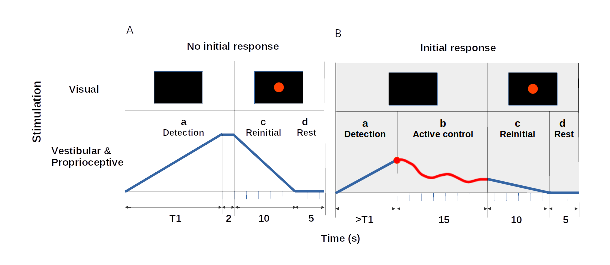
\includegraphics[width=0.9\linewidth]{figures/figure2.eps}
%\end{center}
%\caption{Experimental event timeline examples. Timeline A occurred when the participant did not respond in phase A, it consisted of three phases: (A Detection) motion stimulation of the cabin using a smoothed ramp forcing function, (C Reinitialization) cabin reinitialization to the initial orientation or position, (D Rest) cabin and participant at rest. Timeline B occurred when the participant responded in phase A, the four phases consisted of: A Detection, (B Active control) participant active control, C Reinitialization, D Rest. For both timeline A and B, visual and vestibular stimulation was given during each phase. The blue and red lines are position-based trajectories. The blue line denotes automatic robotic movement of the simulator cabin along one axis per trial, and the red line denotes the stimulus plus the participant’s movements to compensate for the perturbation. T1 denotes the maximum allowed stimulation time per trial with respect to each axis and speed, if initial detection was not made within T1s the experimental phases followed as depicted in timeline A. If the joystick was moved within T1s, an initial response was registered and experimental phases occurred as depicted in timeline B.}
%\label{fig2}
%\end{figure}
% --------------------

% --------------------
% Two figures stacked to make the figures larger and easier to see
% --------------------
\begin{figure}[htp]
\begin{center}
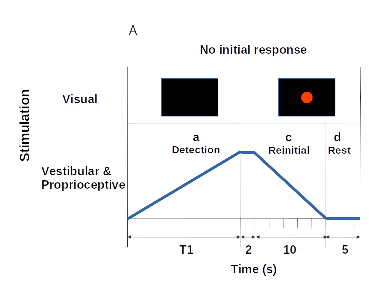
\includegraphics[width=0.9\linewidth]{figures/figure2A.eps}
\end{center}
\end{figure}

\begin{figure}[htp]
\begin{center}
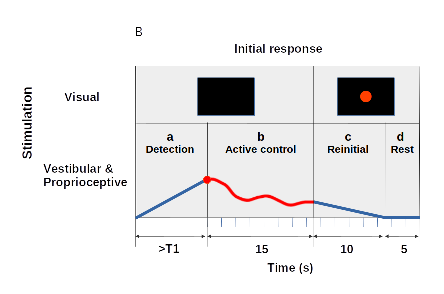
\includegraphics[width=1.0\linewidth]{figures/figure2B.eps}
\end{center}
\caption{Experimental event timelines for when participants did not respond during phase a (Timeline A) and when participants did respond (Timeline B).}
\label{fig2}
\end{figure}
% --------------------

\begin{itemize}
\item Phase a detection: A smoothed ramp-forcing function, where the rate of displacement was unknown to the participants, slowly and continuously perturbed one of the three rotational or translational axes of the simulator cabin at a sub or sup rate. The acceleration profile was the second derivative of the position trajectory. Position trajectories are shown by the blue and red lines in Figure \ref{fig2}. During phase a participants were tasked to perform ``initial detection", which consisted of identifying the axis and direction of the felt perturbation and manipulating a joystick replicating actual aircraft controls (Thrustmaster Hotas Warthog joystick), shown in Figure \ref{fig1}B, in the opposite direction of the stimulus. Participants had 15-20s to detect motion depending on the condition, denoted by T1 in Figure \ref{fig2}, which corresponded to the cabin reaching the maximum allowed cabin displacement for a particular axis and direction. T1 was different for every axis and experiment because sub and sup rates were different for each experiment and the physical cabin displacement range was different for each axis. In particular, the rotational experiment had slightly longer stimulation times than the translational experiment because the sub and sup rates were slower and the available cabin displacements in the RO, PI, and YA orientations were larger than the available translational displacement ranges. If the participants did not respond within T1s during phase A, the cabin automatically displaced along one of the three axes as the ramp function increased until it reached T1s, where the ramp function maintained a zero slope causing the cabin to remain stationary for 2s.
\item Phase b active control: If participants responded within T1s during phase A, phase B active control began and they had 15s to maintain the simulator orientation or position stably at the initial location by counteracting the perturbation; phase B was a vestibular dead-reckoning task. No visual stimulation was present; thus, the participants could rely only on vestibular and proprioceptive cues.
\item Phase c reinitialization: A red dot appeared on the screen instructing participants to release the joystick and rest, while the cabin automatically returned to the initial starting location within 10s.
\item Phase d rest: The cabin remained stationary at the starting location for 5s in order to avoid possible over-stimulation or after-effects.
\end{itemize}

\indent \hl{In summary, the shortest and longest trials were approximately 32s and 50s respectively. The shortest trial length occurred when the participant immediately responded within 1-2s (2s+15s+10s+5s) or did not respond with T1 equaling 15s ((15s+2s)+10s+5s), the longest trial length occurred when the participant responded just before T1 with T1 equaling 20s (19.9s+15s+10s+5s).} Both experiments administered 42 trials: 12 familiarization practice trials and 30 experimental trials. During the familiarization practice phase, unique experimental condition combinations were given, where each of the three axes was stimulated in negative or positive directions at sub or sup speeds. Similarly, the experimental phase consisted of 30 randomized trials, in which 15 trials with unique experimental conditions were repeated twice: five direction-speed conditions (negative sup, negative sub, no-movement, positive sup, positive sub) for each of the three axes (RO/LR, PI/FB, YA/UD). No-movement trials were included as sham trials to encourage the participants to remain active.

\subsection{PARTICIPANTS}
The EuroMov Institutional Review Board (IRB) at the University of Montpellier approved that the scientific objectives and organization of both experiments (IRB-EM rotational: 1703B, IRB-EM translational: 1704B) were safe and appropriate for human participation. The EuroMov IRB committee rules and regulations are in accordance with the 1964 Declaration of Helsinki and its later amendments. Eighteen and 14 healthy volunteers with normal or corrected vision gave informed consent before participating in the rotational and translational tasks respectively (males and females, $32\pm10$ years old); four of the 32 participants reported having novice time-limited piloting experiences lasting less than 40 hours. Four of the 18 rotational and four of the 14 translational participants were over the age of 40 years. The participants who performed the rotational experiment were not the same than those who performed the translational experiment. Therefore, there was no confounds due to experimental ordering, learning, carryover, or fatigue. The same participant population, university students, and staff, was used for both experiments; therefore, it is likely that both experimental populations were similar.

\subsection{EXPERIMENTAL PROTOCOL AND MOTION SIMULATION SYSTEM}
The experiment took approximately 90 min and consisted of four sections (1) arrival, questionnaires, and instruction; (2) familiarization; (3) active control of rotational or translational stimulation; and (4) questionnaire and debriefing. After describing the experimental task and completing the questionnaires, participants were securely installed using the safety harness and communication headphones, as shown in Figure \ref{fig3}A. They were asked to moderately move the joystick in one axis direction at a time while compensating the unknown perturbation. Participants were reminded to maintain the cabin at the initial trial position or orientation, fixed at a steady centered pose, by compensating the motion stimulus. Participants were free to adopt their own strategy to perform the task, both in terms of response speed and of exploration behavior. In order to replicate a realistic flight scenario, the participants were free to move their head and body, looking and/or fixating where they wished, as long as it did not interfere with the task. The fact that the head was left unrestrained is considered undesirable, causing erroneous motion detection due to conflicting self-generated sensory information, and thus rarely performed in traditional motion perception experiments. However we considered it ecologically innovative because it replicated human response under realistic flight circumstances, allowing for a more realistic SD dataset. Once the participant was installed in the cabin, the cabin door was closed and all communication between the participant and experimenter was performed via a camera interface system that facilitated two-way auditory communication. The camera system also provided the experimenter visual feedback of the participant's upper body. The experimenter visually monitored the well-being of the participants, and confirmed participant's feelings of illness auditorily; the experiment ended if the participants reported physical illness.

% -------------------- Figure 3 --------------------
\begin{figure*}[htp]
\begin{center}
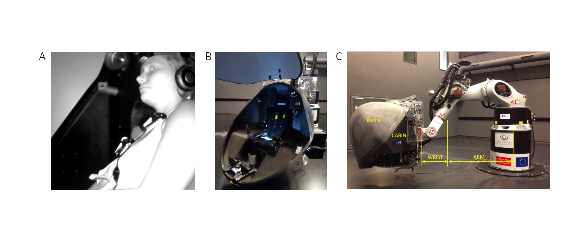
\includegraphics[width=1.0\linewidth]{figures/figure3.eps}
\end{center}
\caption{Motion simulator apparatus and installation; A and B show the experimental simulator cabin with and without a seated participant respectively. C shows an exterior view of the six-axis iMose motion simulator, consisting of the participant cabin and the robotic arm.}
\label{fig3}
\end{figure*}
% --------------------

\indent The motion simulation system that provided sensory stimulation, iMose, consisted of a 6DOF position-controlled KUKA-based motion simulator system (KR 500-3 MT adapted by BEC GmbH motion simulators, KUKA Roboter GmbH, Germany) and a local area network of three 1independent workstations \cite{Denquin_2021_LAF}, \cite{Landrieu_2017_Timetocollision}, \cite{Bellmann_2011_DLR}. Figures \ref{fig3}B and 3\ref{fig3}C show the interior and exterior of the simulation system, data was transferred between the simulator and workstations at 250 Hz on a private network using UDP. Workstations 1 and 3 were located in the experimenter control room; workstation 1 generated motion for the robot using a MATLAB/Simulink control interface program (MATLAB and Simulink Toolbox Release 2009, The MathWorks, Inc., Natick, Massachusetts, USA). Workstation 2 was fixed to the simulator cabin, and it administered the red dot or black visual screen and recorded the streamed user-controlled joystick signal. Workstation 3, using Labview, served as the experimenter’s user control interface to start and stop the experiment and collect experimental data without causing information delays between the workstations.

\indent Two questionnaires were administered before the experimental phase: a claustrophobia assessment \cite{Radomsky_2001_Claustrophobia}, \cite{Radomsky_2006_Claustrophobia_CLQ} and SSQ \cite{Kennedy_1993_Simulator}, \cite{Bouchard_2007_SimulatorSickness}. All questionnaires were administered in the native fluently spoken language of each participant (French or English). The claustrophobia questionnaire consisted of two sections: the first section measured fear of suffocation (14 questions) and the second section assessed fear of restriction (12 questions). The claustrophobia questionnaire was used as a screening method to assess whether participants could enter the simulator and perform the task relatively stress-free; participants who scored 40 points or lower, indicating that they were not claustrophobic, were initially recruited, and participants scoring higher than 40 were recruited last. For both the rotational and translational experiments all participants scored “non-claustrophobic”, rotational results were mean=10.94, max=38, min=0 and translational results were mean=8.77, max=9, min=0. The SSQ consisted of 16 questions and measured the participant’s general physical state, evaluating nausea, ocular motor, and disorientation sub-scales. The SSQ was administered before and after the experiment to measure the effects of the experiment in terms of disorientation.

\section{ANALYSIS}
As previously mentioned, the goal of this study was to create a realistic flight dataset of moments of disorientation and non-disorientation measured by joystick motion, and then identify the best methods to predict SD using ML and DL methods. The analysis methodologies were as follows: 1) verifying the correctness and authenticity of the dataset, 2) evaluating ML and DL modeling parameters for SD classification using three metrics, and 3) statistically correlating physical with perceptual disorientation to confirm whether other possible measures besides joystick could convey markers for the occurrence of human SD-state. Python was used for all analyses, using numpy, pandas, scipy, pywt, tensorflow, scikit-learn, seaborn, plotly, and matplotlib (Python 3.9, Python Software Foundation, Fredericksburg, Virginia, USA).

\subsection{VERIFICATION OF SIMULATION DATASET}
\label{VERIFICATION_OF_SIMULATION_DATASET}
All trials, familiarization and experimental trials, were used in data analysis to maximize data usage. The simulator system motion and participant joystick responses were down-sampled from 250 Hz to 10 Hz for data analyses, such that only relevant human motor movements were considered; literature has shown that human hand and arm movements do not exceed frequencies of 10 Hz \cite{Shadmehr_2004_Computational}.

\indent Data standardization pre-processing analysis was performed to ensure that the data was collected properly. Data standardization consisted of two-steps: 1) numerical confirmation of experimental settings, and 2) numerical confirmation of the experimental design. In the first step, four items were checked for correctness using both joystick and cabin motion data: experimental event matrix per trial, joystick and cabin directional control convention, joystick margin needed to command cabin motion, and start-stop time of phases A and B per trial. In the second step, the motion and timing of the cabin with respect to joystick motion was checked for correctness. The robotic simulator performed motion stimulation in real time using a real-time Linux kernel, with a MATLAB/Simulink input layer, to capture responses with minimal delay. Despite the advantage of rapid response synchrony, real-time systems are prone to having system delays that can influence functional timing and communication between tasks; real-time functioning refers to the order in which numerical tasks are executed using the available computer resources. Therefore, the rotational and translational experiments had trials where system delays imperceptibly influenced the robotic trajectory and/or the participant's ability to respond correctly via the joystick. Due to these slight processing and thus execution errors that are due to the real-time functionality of the motion simulator, it was necessary to remove all trials that had frequency or joystick-cabin related defects such that experimental defects were not confounded with participant response. The following defects were checked in the second step of data standardization:
\begin{itemize}
\item temporal gaps in data,
\item trials where phases A and/or B were shorter than the minimal expected trial length of 17s, denoting the system sampling frequency was faster than desired,
\item trials where joystick motion was sufficient but the cabin insufficiently moved,
\item delays longer than 5s between joystick and cabin movement.
\end{itemize}

\indent The majority of trials that were removed were due to fast or slow system frequency sampling rates, thus discarding trials that had recorded timestamps less or more than 17 s or 50s respectively. The second reason for discarding trials was due to the fact that the cabin did not respond within a few seconds after joystick movement, or the cabin motion axes and direction was incorrect with respect to joystick motion. In total, 40\% of rotational and 50\% of translational trial data was removed from the analysis. Errors were expected as the system was a new experimental test platform where many computers needed to operate in synchrony. Data standardization was the only step that removed trial data, trials that passed data standardization were used in data analysis.

\subsection{RESPONSE CATEGORIZATION}
Detection of correct stimuli was categorized into ten possible categories based on the selection of axis and axial direction. Figure \ref{fig4} depicts a flowchart and possible participant choices based on response movements. The blue squares indicate the experimental trial type: the presence of motion stimuli denoted by ``Movement" and no presence of motion stimuli denoted by “Sham". For “Movement" activity, the green squares indicate participant response activity such that “1-3 axes” means that the participant moved the joystick on one or more axes and “No axes" means that the participant did not move the joystick. The yellow diamonds denote the decision process based on the question asked within the diamond. For example, for “Movement" activity where the participant responded using one or more joystick movements, the following question is posed: “Is the stimulus axis the same as the axis in which the participant initially moved the joystick?”. If yes, the axis was noted as correct, and the initial direction was confirmed in a similar manner. For example, “Did the participant initially move in the opposite direction of the stimulus direction?”. The red numbers indicate the total number of possible categories based on the logical progression of performing the task correctly, first finding the correct axis and then finding the correct direction to counteract the vestibular stimulus.

% -------------------- Figure 4 --------------------
\begin{figure}[htp]
\begin{center}
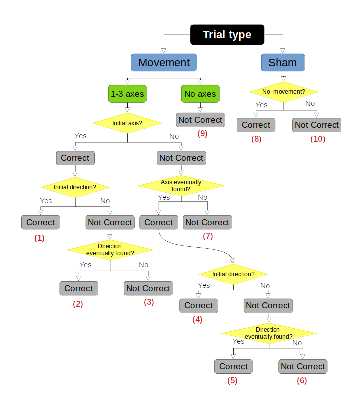
\includegraphics[width=1.0\linewidth]{figures/figure4_2.eps}
\end{center}
\caption{Flowchart of selection process for detection performance categories, where correct response categories 1, 2, 4, and 5 denote non-SD occurrence and wrong response categories 3, 6, 7, and 9 denote SD occurrence.}
\label{fig4}
\end{figure}
% --------------------
The ten detection performance categories were reduced to four categories:
\begin{itemize}
\item Initially Correct axis and direction: trials in which the first response was with the correct axis and direction (IC: Category 1)
\item Eventually Correct axis or direction: trials where the first response was with an incorrect axis or direction but the correct axis and direction was found (EC: Category 2, 4, and 5)
\item Never Correct: trials where participants acted on the joystick but never found the correct axis and/or direction (NC: Category 3, 6, and 7)
\item No response: trials in which participants did not respond (NR: Category 9). 
\end{itemize}
Categories 8 and 10 corresponded to the no-movement sham trials and were not used in the analysis.

\subsection{MOTION DETECTION AND PERFORMANCE SUMMARY}
\label{MOTION_DETECTION_AND_PERFORMANCE_SUMMARY}
The normalized response count and Reaction Time (RT) per detection performance category were quantified for each axis and speed condition. The normalized response count was the adjusted count per response category, with respect to the given number of trials multiplied by participants; the total trial count per participant was 36, excluding sham trials. The total trial count per participant was adjusted to 36, such that the interpretation of results would be consistent with the experimental design. Participants had fewer total trials than 36 trials because trials that did not follow the experimental design were removed during the data standardization step mentioned in Section \ref{VERIFICATION_OF_SIMULATION_DATASET}. RT was the time that the participant used to find the correct axis and direction. The 95\% confidence interval per axis was calculated to determine which detection performance categories were significant. Detection performance categories above the lower confidence interval were evaluated further. Significant and corresponding detection performance categories were compared for the speed and axis.

\indent The Kolmogorov-Smirnov (KS) test was used to evaluate whether to use a parametric or non-parametric two-sample comparison test for within-axis and across-axis comparisons. All test evaluations resulted in non-parametric distributions; therefore, only non-parametric tests were used. Two non-parametric tests were used to evaluate comparisons: Wilcoxon signed-rank distribution test and Wilcoxon rank-sum distribution test \cite{Foundation_2013_python}. Uneven two-sample non-parametric test data vectors were compared using the Wilcoxon rank-sum test. However, the Wilcoxon signed-rank test required that equal length vectors be compared, thus shorter length vectors were padded with NaN values to preserve the equivalent number of samples with respect to the longer vector and the distribution of the shorter length vector. Statistical p-values are reported using the following standardized significance levels: the Bonferroni required value of 0.0167 for two test comparisons, 0.05 for single test comparisons, and 0.001 for strongly significant one or two test comparisons. A participant detection performance rank score was created to compare overall participant detection performance with perfect performance. The performance rank score was calculated per subject across trials, per experiment, where

\begin{equation}
Rank~score = 2 \cdot (IC~count) + (EC~count)
\label{eqn_rank_score}
\end{equation}

The rank score equation weights were arbitrarily chosen such that the equation formulation was most simplistic; RT was not considered in the rank score because rotational and translational experimental stimulation timings were different and thus non-comparable. IC performance was the desired behavior for the task so a weight of two was given to each IC trial. EC was also desired task behavior because participants were able to eventually find the correct axis and direction, however mistakes were made, thus a weight of one was given to each EC trial. NC and NR performance trials were not the desired task behavior so they were given no credit. Thus a rank score of 72 corresponded with perfect performance, where IC detection was performed for all 36 motion stimuli trials. Finally, the rank score was used to divide participants into three final categories in order to summarize performance with respect to each experiment. Mean and standard deviation of participants' rank score per experiment were calculated, such that participants were divided into best, average, and worst categories if their rank score was greater, within, and lower than one standard deviation from the experimental participant mean respectively.

\subsection{CLASSIFICATION MODELS, FEATURE \& LABEL CREATION}
ML and DL, sequential and spatial/parallel modeling methods were selected for SD classification. Modeling performance metrics were compared using time, frequency, and time \& frequency features. As mentioned in subsection XXX, it was of interest to understand whether time and/or frequency joystick derived features could be better predicted using a sequential versus spatial/parallel model architecture. The sequential architecture models included Support Vector Machine (SVM) and Long Short Term Memory (LSTM). Spatial/parallel models were 2D CNN and Transformer; the Random Forest (RF) subspace model architecture was additionally implemented for bench-marking for this novel dataset. Detection classification was performed for each speed condition (sub, sup), and across axis conditions. Feature selection was motivated by two factors: the modeling analysis desire to compare time and/or frequency signal influences on model architecture, and to exploit the human movement domain principle that humans regulate velocity and acceleration to perform a position-based motion.

The six explored types of joystick features were:
\begin{itemize}
\item time-only: time-series joystick signal in sequential order,
\item time-only: time-series joystick signal in non-sequential order,
\item time-only: k-means clustering using all position, velocity, and acceleration as feature space points.
\item frequency-only: five frequency pattern sublevels of the discrete time wavelet transform using the symlets 5 mother wavelet\cite{Nedorubova_2021_CWT_CNN_HumanActivity},
\item time \& frequency: flattened short-time fast Fourier transform (fft),
\item time \& frequency: flattened continuous wavelet transform using the Mexican hat mother wavelet as reported in \cite{Nedorubova_2021_CWT_CNN_HumanActivity},
\end{itemize}
For each of the six types of features, three human movement signal transformations were considered; position, velocity, and acceleration representations of the experimental hand control response using the velocity-controlled joystick. In total 29 time and frequency features were calculated.

Three types of semi-supervised labels were created for predicting disorientation:
\begin{itemize}
\item Lenient: mistakes are allowed to be made thus IC and EC categories were labeled as ‘non-disoriented’ and NC and NR were labeled as disorientation,
\item Strict: no mistakes are allowed where IC was labeled as not disorientation and EC, NC, and NR were designated as disoriented,
\item Complex: a multi-label depicting SD via NC and NR responses, mild-SD using EC responses, and non-SD using only IC responses.
\end{itemize}
The purpose of testing different labels was to understand how to best define SD from the intrinsic organization of the data; better predicting models using a certain label implies that the data is best structured for that label. We compare our data-driven definition of SD with the current functional definition of SD \cite{Newman_2007_SD}.

\subsection{CLASSIFICATION MODEL EVALUATION}
Average 5-fold cross validation test prediction accuracy and ROC-AUC measures were used to evaluate ML model performance. Accuracy measured the true positive (TP) and true negative (TN) counts over the total number of samples; a value of 1 and 0 correspond to 100\% and 0\% correct prediction. Accuracy only gives information about how well the model approves data, but not about how well the model rejects data. Therefore, the familiar ROC- AUC measure was used to evaluate both classification acceptance and rejection performance. ROC-AUC is the area under the false positive rate (FPR), shown in equation (\ref{eqn_fpr}), versus the True Positive Rate (TPR), shown in equation (\ref{eqn_tpr}),

\begin{equation}
Accuracy = \frac{TP+TN}{TP+TN+FP+FN}
\label{eqn_accuracy}
\end{equation}
where FP and FN correspond to false positive and negative counts, respectively. 

\begin{equation}
FPR = \frac{FP}{FP+TN}
\label{eqn_fpr}
\end{equation}

\begin{equation}
TPR = \frac{TP}{TP+FN}
\label{eqn_tpr}
\end{equation}

\noindent An ROC-AUC score of one indicates perfect prediction of all labeled classes, whereas a score of 0.5 or lower indicates that prediction of all labeled classes was poor with chance level performance or lower. ROC-AUC was needed in addition to accuracy to determine if FP values were balanced with TP values, ensuring that the SD model could accurately reject and accept the data \cite{Burkov_2019_ML}.

\indent Finally, feature importance was of interest because each feature contained distinct information about disorientation. It was of interest to understand which feature/s could convey the most informative information about the occurrence of perceptual disorientation. Feature importance was calculated such that each feature was shuffled individually and model accuracy was calculated for each shuffled feature. Unshuffled model prediction accuracy was subtracted with each of the shuffled feature prediction accuracy scores. The change in prediction accuracy for each shuffled feature was ranked, such that the feature with the largest change in prediction accuracy was considered the most important feature. Feature importance was calculated using scikit-learn's permutation importance function, and manually calculated for Tensorflow models. Individual metric comparisons, of the three metrics, were evaluated using the same Wilcoxon signed-rank or rank-sum tests where p < 0.05 and p < 0.001 were considered significant and strongly significant respectively; only non-parametric tests were used because the KS test reported non-parametric distributions.

\subsection{PHYSICAL DISORIENTATION}
Detection performance categories were related to only the SSQ disorientation sub-scale, not the combined SSQ score, because the task was related to disorientation with respect to motion detection \cite{Kennedy_1993_Simulator}, \cite{Bouchard_2007_SimulatorSickness}. Physical disorientation was monitored before and after the experiment using the SSQ disorientation sub-scale, such that the difference in before and after measures were attributed to the experienced task; SSQ disorientation difference equaled the disorientation score before the experiment minus the score after the experiment.

Negative SSQ disorientation difference meant that the task made the participant disoriented (e.g., they felt better before), and positive SSQ disorientation difference meant that the task rendered the participant less disoriented (e.g., they felt better after). Physical disorientation for accurate and non-accurate motion detection performers were compared, to quantify whether physical disorientation report could also be a marker for SD, like the perceptual joystick. Again, Wilcoxon signed-rank or rank-sum non-parametric distribution tests were used to evaluate comparisons, as the KS test only found non-parametric distributions. The mentioned statistical p-value reporting convention was used.

\section{RESULTS}
For both rotational and translational experiments, participants’ detection behavior was quantified using the detection performance categories in terms of count and initial RT with respect to stimulation speed and axis; no significant differences were found between positive and negative axial directions thus directional differences were not considered. As previously mentioned, human motion detection ability of self-motion along axis and axial directions are often reported in terms of motion detection threshold \cite{Valko_2012_Vestibular}, \cite{Hartmann_2014_Direction}, \cite{Karmali_2017_Multivariate}. A motion detection threshold is registered from a self-report that motion was felt along a specific axis and direction for a specific motion stimulus frequency. Results are typically displayed in terms of mean detection count across or per subject for many stimulus motion frequencies, where count results are grouped by successful and unsuccessful detection. We performed the same analysis presentation for our two sub and sup stimulus frequencies, displaying results in terms of count, mean count, and RT across participants, where count and RT results are grouped by detection performance categories.

\subsection{MOTION DETECTION PERFORMANCE}
Figure \ref{fig5} shows the normalized summed count (top row), normalized mean count (middle row), and mean RT (bottom row) per detection performance category, across participants for RO, PI, YA, LR, FB, and UD axes and sub \& sup speed conditions, for both rotation and translation. The top row shows the normalized summed count per detection performance category for each axis and speed condition. For rotation, the summed bars in the top row are equal to 648, which corresponds to the 18 participants multiplied by 36 trials. The top row represents the distribution of total trial responses per response category. Similarly, for translation, the summed bars in the top row are equal to 504 which corresponds to the 14 participants multiplied by 36 trials. The middle row shows the mean count of the same normalized count data across participants. The mean count represents the frequency of selecting a response category across participants. \hl{It was necessary to show both mean and total selection count because average axis selection count can not be clearly understood from the total axis selection count; total count gives information about overall participant response and average count gives information about participant tendencies.} The bottom row displays the mean RT taken to detect correctly, thus only IC and EC response categories are shown. Bars without error bars indicate a single sample value, or several participants had the same count value. Single-sample bar values may exist due to data elimination during the rigorous standardization process. Wilcoxon signed-rank test and rank-sum tests were used to determine significance such that significant and slightly significant relationships were represented by (* within axis comparison of sub and sup, ** across axes comparison). Bonferroni correction: p < 0.0167 was used as the significance threshold. Detection performance categories above the lower confidence interval, denoted by the solid red line, were considered for statistical comparison across subjects for categories within (e.g.; sub vs. sup) and across axis (e.g.; RO sub vs. PI sub) conditions.

% -------------------- Figure 5 --------------------
\begin{figure*}[htp]
\begin{center}

\includegraphics[width=1.0\linewidth]{figures/figure5.eps}
\end{center}
\caption{Normalized summed count (top row), normalized mean count (middle row), and mean RT in seconds (bottom row) per detection performance category, axis, and speed for rotational and translational stimulation.}
\label{fig5}
\end{figure*}
% --------------------

\subsubsection{DETECTION: SPEED COMPARISON (WITHIN AXIS CONDITION)}
There was a slightly significant sub versus sup count difference for the most counted detection performance category for the RO and PI axes, where sup speed resulted in a higher count than sub speed (RO count EC sup vs sub: KS: non-normal distribution, signed-rank: p < 0.001, rank-sum: p < 0.026, n=13; PI count IC sup vs sub: KS: non-normal distribution, signed-rank: p < 0.08, n=18). Slight significance is denoted in the top row of Figure 5, with a single star in purple and blue. There was a similar trend for the YA axis, where the most counted detection performance category, IC, had a higher sup count than sub count. This demonstrates that participants were more accurate at sup speed than at sub speed, regardless of the motion stimulation axis or direction. No significant differences between sub and sup speeds were found in the translational experiment. However, there was a trend for all axes where the most counted detection performance category had higher sup counts in comparison to sub counts. For example, the EC detection performance category for the LR and FB axes and the IC detection performance category for the UD axis had greater sup counts than sub counts. Translational motion sub and sup speed differences were less apparent than in rotational motion due to inner-ear stimulation differences. Reduced speed detection in translational motion are likely attributed to less semi-circular stimulation and delayed otholic signaling in comparison to rotational motion \cite{Angelaki_2008_Vestibular}. Therefore, we suspect that more data was needed for differences to become statistically significant.

\indent Regarding RT differences for the rotational experiment, some detection performance categories had significantly lower RTs for the sup than the sub speed condition. For RO and PI axes, the RT for the most counted detection performance category was significantly lower for sup speed in comparison to sub speed (RO RT EC sup vs sub: KS: non-normal distribution, signed-rank: p < 0.001, rank-sum: p < 0.001, n=66; PI RT IC sup vs sub: KS: non-normal distribution, signed-rank: p < 0.001, rank-sum: p < 0.001, n=65); significance is denoted in the bottom row of Figure 5 with a single star in purple and blue. In summary, we demonstrate that faster sup motion caused more accurate and faster motion detection than slower sub motion. This result has been reported in motion detection literature, thus confirming that the experiments were performed correctly and that the dataset accurately represented human response \cite{Valko_2012_Vestibular}, \cite{Hartmann_2014_Direction}.

\subsubsection{DETECTION: AXES COMPARISON (ACROSS AXES PER SPEED CONDITION)}
The same speed condition and successful response categories denoted by IC and EC were compared across axes, in order to identify task difficulty with respect to the axis, and thus demonstrate that our experimental results were in alignment with psychophysical motion detection findings. Whole-body motion detection literature shows that RO and PI are easier to detect than YA and translational motion. According to a report RO and PI detection thresholds were statistically similar for novices and experts \cite{Hartmann_2014_Direction}. Additionally, RO was reported to be easier to detect than LR, UD, and YA in both non-vestibular and vestibular dysfunction participants \cite{Valko_2012_Vestibular}. Table \ref{table1} depicts significant differences in response count and mean RT for specific speed and axis categories. Category 1 and 2 represent categories with high count or fast RT and categories with low count or slow RT respectively; the first and second p-values correspond to the signed-rank and rank-sum test respectively. Listing significant differences allowed us to rank axis conditions, with respect to motion detection ease and difficulty, and then compare the ranked list with literature reports to confirm correctness of experimental stimuli. Table \ref{table1} shows that, in alignment with literature reports, we similarly found that RO, PI, and FB axial motions were easier to detect than YA, with dependence on speed when considering only correct responses. In particular, successful response category counts for both RO and PI at sup speed were significantly higher than those for YA, and for sub speed FB and PI had significantly higher counts than YA.

\begin{table}[h]
\caption{COUNT AND RT COMPARISONS FOR COMBINED IC \& EC RESPONSE.}
\label{table1}
\centering
\begin{tabular}{C{15pt}C{40pt}C{40pt}C{90pt}}
\hline
\multicolumn{1}{c}{} & \multicolumn{2}{c}{Speed \& axis} & Significance\\
\hline
\multicolumn{1}{c}{} & \multicolumn{1}{c}{Category 1} & \multicolumn{1}{c}{Category 2} & \multicolumn{1}{C{90pt}}{(KS: non-normal, signed-rank, rank-sum)}\\
\hline
Counts & sup RO & sup YA & p < 0.001, 0.0167, n=20\\
 & sup PI & sup YA & p < 0.001, 0.0167, n=20\\
 & sub FB & sub YA & p < 0.001, 0.0167, n=22\\
 & sub PI & sub YA & p < 0.001, 0.001, n=22\\
\hline
mean RT & sup RO & sup YA & p < 0.001, 0.001, n=67\\
 & sub PI & sub YA & p < 0.001, 0.001, n=67\\
 & sub FB & sub YA & p < 0.001, 0.001, n=41\\
\hline
\end{tabular}
\end{table}

\indent Moreover, our results showed functional differences between the RO, LR, \& FB and PI, YA, \& UD tasks. During PI, participants mostly detected correctly (IC) and rarely when they did not detect correctly, they eventually or never corrected. Again in YA, participants often detected correctly (IC), but when they did not detect correctly they did not feel any motion (NR). Similarly in UD participants often detected correctly (IC), and when they did not detect correctly they often eventually corrected; IC was more prevalent when speed was fast. Whereas in RO, LR, and FB, participants could not initially detect the correct axis and/or direction, but they could eventually find the correct axis after several mistakes.

\indent Lastly, task difficulty for within rotational and translational stimulation appeared to be correlated with longer RT. As mentioned in Section \ref{EXPERIMENTAL_DESIGN}, participants were stimulated slower in the rotational task than in the translational task; thus, RT was different for the rotational and translation tasks and were not compared. The second portion in Table \ref{table1} labeled RT, shows the significant within experiment comparison across axes for only correct responses. For the rotational task at sup speed, RO and PI had faster RT than YA indicating that participants needed less time to detect motion for RO and PI. Similarly, for the translational task at sup speed, FB had significantly faster RT than UD.

\subsection{MOTION DETECTION PERFORMANCE RANK}
Including both rotational and translational tasks, the highest rank score was 55 and the lowest score was 11. On average, participants received a rank score of 37. Therefore, the best performer, regardless of rotation or translation, achieved $(55/72) \cdot 100=76.3\%$ accuracy for the task. The average performer was only able to achieve $(37/72) \cdot 100=51.38\%$ accuracy for the task. The same task accuracy statistic was calculated for sub and sup conditions individually, for both rotation and translation experiments, and similar results were found, as shown in Table \ref{table2}. Table \ref{table2} shows the experimental performance accuracy per speed condition using the performance rank measure. All percentages were calculated by dividing by 36 trials.

\begin{table}[h!]
\caption{DETECTION PERFORMANCE RANK PER SPEED CONDITION.}
\label{table2}
\centering
\begin{tabular}{C{50pt}|C{30pt}C{40pt}C{25pt}C{40pt}}
\hline
Rank & Rot sub & Trans sub & Rot sup & Trans sup \\
\hline
Best & 83.3\% & 75\% & 80.5\% & 77.7\% \\
Average & 47.2\% & 55.5\% & 55.5\% & 58.3\% \\
Worst & 11.1\% & 0\% & 30.5\% & 25\% \\
\hline
\end{tabular}
\end{table}

These rank statistics show that the detection task was challenging for the average person, regardless of the experimental conditions, but it was not impossible to perform with reasonable success. The participant distribution count for the rotational experiment was five best performers, 11 average performers, and two worst performers. Similarly, the participant distribution count for the translational task was as follows: two best performers, 11 average performers, and one worst performer. The rotational and translational participant distribution counts for best, average, and worst performance were similar, showing that both tasks were similarly challenging in terms of motion detection. Therefore, translational detection may not be more difficult than rotational detection in realistic environments.

\subsection{SD CLASSIFICATION}
TO BE ADDED


\subsection{MOTION DETECTION PERFORMANCE AND PHYSICAL DISORIENTATION}
Twenty of the 31 participants did not feel any difference in terms of physical disorientation during the entire experiment. Considering the performance rank score mentioned in Section \ref{MOTION_DETECTION_AND_PERFORMANCE_SUMMARY}, approximately 1/3 of the average detectors, 1/3 of the best detectors, and 2/3 of the worst detectors experienced physical disorientation. The 2/3 worst detection ratio is reported for completeness; however this measure is disregarded because it is based on only three participants. Thus, 1/3 of the population felt physical disorientation regardless of performance.

\indent To investigate whether there was a relationship between physical disorientation and detection performance, the detection performance of the 12 participants who reported physical disorientation was evaluated; see Table \ref{table3} for a percentage of their summed trial performance per category per SSQ difference report. For instance, a participant who reported a before and after SSQ score of six and four respectively would have their trial performance category counts, of eight EC and six IC trials, associated with an SSQ disorientation difference score of negative two. Table \ref{table3} shows the motion detection response category per reported SSQ disorientation sub-scale difference for both the rotational and translational experiments. Performance category percentage values across SSQ scores sum to 100\%. Negative and positive SSQ values denote that the participant felt better before and after the task respectively. The bold percentages corresponding to negative SSQ values for categories EC and NC highlight that more negative physical disorientation was present in unsuccessful initial attempts to detect motion. Table \ref{table3} demonstrates that more negative physical disorientation was observed for unsuccessful initial detection response categories EC and NC, than for IC successful initial detection response or no response. The negative and positive SSQ disorientation differences per response category were summed respectively, to evaluate significance between IC negative and NC or EC negative. Physically disoriented best performers (IC) did not report significantly less physical disorientation than poor performers.

\begin{table}[h!]
\caption{SSQ DISORIENTATION SUB-SCALE PER MOTION DETECTION PERFORMANCE CATEGORY}
\label{table3}
\centering
\begin{tabular}{c|ccccccc}
\hline
& \multicolumn{7}{c}{\centering SSQ (\%)}\\
Category & -5 & -3 & -2 & -1 & 1 & 2 & 4\\
\hline
IC (1) & 5.4 & 8.4 & 17.8 & 23.6 & 24.5 & 8.9 & 11.5\\
EC (2,4,5) & 10.1 & 12.0 & 29.0 & 26.6 & 14.1 & 2.8 & 5.4\\
NC (3,6,7) & 10.3 & 2.7 & 38.5 & 26.3 & 5.2 & 11.5 & 5.5\\
NR (9) & 0 & 3.4 & 20.8 & 18.7 & 26.0 & 21.8 & 9.4\\
\hline
\end{tabular}
\end{table}

\indent In summary, we found no significant relationship between physical disorientation and motion detection. There was only a trend that EC and NC performers, who felt physical disorientation, felt better before the task than after. This implies that participants became fatigued while trying to perform the task, when detection was not easy for them. For IC performers who experienced physical disorientation, there was no trend in terms of feeling better before or after. Implying that participants who could detect easily, felt discomfort for other reasons not related to the experiment. There was a slight trend for NR performers that felt physical disorientation, such that they felt better after the task than before. Showing that participants who did not respond, became comfortable and relaxed in the dark experimental setting.


\section{DISCUSSION}

TO BE ADDED
% Highlight the findings


% List the advantages of the study with respect to past research from various research field


% Explain the limitations of our work.


\section{CONCLUSION}
% ------------------------------------
% Restate the goal of the work within the scope of the problem statement, our approach to addressing the problem, the significance of our work based on the results
% ------------------------------------
In this comprehensive study on SD, we show that it is possible to isolate, simulate, and recreate realistic aspects of a vestibular feedback dead-reckoning piloting task and predict the occurrence of SD using joystick response as a feature. We demonstrate that SD can be modeled in a generalized manner with respect to task performance (e.g., correct, not correct) and a human behavioral measure which was joystick motion. Using the ML framework of label and feature organization, SD can be predicted accurately for each SD use-case using use-case specific joystick data or non-specific use-case joystick data. Additional, if other human behavioral measures were included as features such as physiological measures, ML classification could include both prediction of SD and prediction of specific use-case. Thus, SD can also be studied and predicted using a data-driven ML task-measurement approach, instead of the widely practiced functional use-case driven approach.

% ------------------------------------
% Summary of the experimental motion detection results
% ------------------------------------
% From a motion detection literature perspective
\indent The generalized experimental design allowed for the collection of perceptual response joystick data during various basic scenarios of vestibular and proprioceptive stimulation; SD or non-SD states were apparent via the joystick response. A crucial data standardization step was used to verify that the simulator system correctly performed the experimental design, removing trials with delays and erroneous motion. The SD-targeted dataset captured known human motion detection trends, demonstrating that the real-time motion simulation environment was fidel despite the functional timing delays \cite{Stoffregen_2003_Nature}. To mitigate functional timing issues, where some events were executed incorrectly before other events, programming events could have been grouped into functional blocks or scripted codes, where similar tasks were executed in synchrony. Known motion detection trends include: a) accurate and faster response for sup speed stimulation in comparison to near below-threshold speed stimulation, b) PI, RO, FB, LR, UD, and YA were the least to most difficult axis tasks, c) longer reaction times corresponded with task difficulty for the respective rotational and translational experiments \cite{Valko_2012_Vestibular}, \cite{Hartmann_2014_Direction}, \cite{Karmali_2017_Multivariate}. Ranking of task difficulty per axis confirms literature reports that there is no sensory advantage for UD detection due to gravity, because the vestibular system compensates for gravity \cite{Valko_2012_Vestibular}. In addition to confirming known motion detection trends, functional differences in motion detection for RO, LR, \& FB and PI, YA, \& UD tasks were observed; where the most counted response for RO, LR, \& FB was EC in comparison to IC for PI, YA, \& UD. It is unclear why participants made more initial mistakes for RO, LR, \& FB than PI, YA, \& UD axes, however perhaps participants relied on more non-vestibular sensory cues (proprioception, tactile, auditory from the simulator motor) and/or had better natural upright posture during certain stimulus motions than others. Perhaps in PI, YA, and UD they relied more on clear vestibular cues because they self-generated less additional motion information from self-motion or joystick interaction, thus allowing participants to either initially detect correctly or not.
It appears plausible that in RO, LR, and FB participants were more likely to generate additional and perhaps conflicting sensory information by naturally tilting or turning the head. It is likely that participants naturally adapted their posture, to be more or less upright, during certain motion stimuli in comparison to others. For example, a slightly left tilted head during pitch motion would more likely induce discomfort than during roll motion, thus encouraging participants to naturally sit upright during pitch stimuli and thus giving them an advantage to detect the motion more clearly. Such functional errors in RO, LR, and FB caused by natural postural behavior could easily escalate the occurrence of spatial disorientation.

% From a global perspective in terms of Data Science or general psychology experimentation perspective
\indent Statistical analysis showed that regardless of experimental conditions, the best performers achieved 76\% detection accuracy and average performers achieved 51\% accuracy. The task may have been difficult because participants were given the freedom to decide on which axis and in what direction the stimulation occurred, as is done in a real-life piloting situation. All participants had very little to no piloting experience, thus our results reflect human motion perception without the influence of piloting experience or training. Thus, the modeling results obtained from this dataset may not be representative of expert piloting behavior, because our novice participants’ responses have more variability than expert piloting responses.

% ------------------------------------
% Summary of classification modeling results
% ------------------------------------
% Short motivation of using ML modeling instead of control theory, from a motion detection experimental persepctive
\indent Using the SD dataset we investigated modeling methods for predicting SD, including statistical analysis, predictive control, and ML. Predictive control has been used to predict motion detection \cite{Soyka_2011_Predicting}; however, ML methods have been shown to be efficient and accurate in finding patterns among different types of data and constructing reusable models for future prediction \cite{Burkov_2019_ML}. Using ML techniques, we investigated parameter tuning selection for the prediction of SD and explained the importance of different parameter selection methods. We evaluated the importance of model construction parameters using test set prediction accuracy and ROC-AUC as a benchmark and comparative measure. Five key model construction parameters were tested: feature quantity, eight model types, dataset conditions, feature type, and semi-supervised label type.

\indent Regarding the number of features in each ML model, no significant difference was found in the prediction accuracy when using all six joystick features, three of the most important features, two of the most important features, or the most important feature alone. Thus, building a model on a single important feature is sufficient to predict SD. However, it is a best practice to use all relevant features for model construction. Decision tree type models (DT, GBC, RF) were superior, to non-decision tree models (SGD, LDA, MLP, GNB, NuSVC) using simplistic features, in test accuracy prediction regardless of the experiment (rot, trans), axis, speed, and semi-supervised label. On average decision tree models had accuracy rates ranging from 0.8-0.99 depending on the model type. These models were able to learn associations between features and labels regardless of semi-supervised label construction. However, non-decision tree models predicted the best when labels were constructed with a binary label instead of a multi-label. Specifically, the lenient label resulted in better prediction than the strict label. On average non-decision tree models with binary labels had accuracy rates ranging from 0.5-0.85. Moreover, specialized models for axis or speed conditions did not outperform models in which all data were used for decision tree models. Whereas, for non-decision tree models, some specialized models predicted better than models in which all the data was used, implying that lower data variability is important for SD prediction using non-decision tree models.

% CONFIRM


%\indent Three main findings were identified during feature importance investigation: 1) decision tree models perform best using constant natural frequency features, 2) non-decision tree model feature importance identified more temporal features as being important than constant natural frequency features, and 3) semi-supervised labels did not influence feature importance for decision tree models however the strict label for non-decision tree models identified only temporal features as being important. When a ML model performs poorly or does not select a feature as being important, it means that the optimization strategy cannot produce a prediction in alignment with the label, using the given feature information. non-decision tree models poorly use features with repeating constant values because the optimization strategies often require feature data point distances to be optimized in a certain manner. Feature data points with the same value do not allow for the optimization algorithms to find optimal maximization or minimization predictions. In hindsight, instead of using constant natural frequency features as a simple categorical-type feature, it would have been more insightful for optimization methods to create a more complex natural frequency feature using wavelets or PCA, and/or features created from a clustering method like kmeans. Despite the fact that decision tree models appear to be more accurate and easier to tune than non-decision tree models, non-decision tree models are useful for data with stationarity and merit the additional time to optimally tune these models. An optimally-tuned non-decision tree model would be able to predict the occurrence of SD while accounting for stationarity trends, like those that occur during the leans SD use-case, while decision tree models are more likely to confuse the trend with SD related behavior.

\indent Finally, the decision to choose a strict or complex label convention versus a lenient label to discern SD depends on the application and the quantity of data available to represent a non-SD state. The strict label was less realistically representative of non-SD, because perfect behavioral data in any task is statistically rare, thus building an accurate model using a strict label convention maybe more challenging. Similarly, for the complex semi-supervised label there was a lack of representative data for each of the SD cases. Over-fitting, where training predictions were higher than test predictions, was observed for both strict and complex labels supporting a lack of data for these labeling conventions. The lenient label, labeling with respect to overall correctness regardless if mistakes are made, was shown to be the best labeling convention as: 1) over-fitting was less observed for our small dataset where test and training predictions were similar, 2) both natural frequency and temporal features were selected as important features thus a diversity of relevant simple patterns were captured. Moreover, prediction accuracy with respect to semi-supervised label construction can be used as a confirmation for how to define SD because semi-supervised means that the label is not 100\% the ground truth. The prediction accuracy of the model construct using the data, conveys missing information about the label based on trends in the data. If a model predicts better with label A than label B it means that label A better matched the existing data structure, thus confirming that label A is likely to be the ideal label for the data. Therefore, applying this idea to the three semi-supervised SD labels. The lenient label is the ideal label convention for modeling SD, with respect to our dataset, because on average both decision tree and non-decision tree models predicted the test data best using the lenient label. A lenient label convention, where SD is defined as never correct or no response, is also in alignment with the definition of SD, where SD is defined as involving successive failures and major performance errors \cite{Newman_2007_SD}.

% ------------------------------------
% Results about the experimental questionnarie as a viable measure for SD
%that measured sickness caused by inner-ear stimulation,
% ------------------------------------
\indent 

One-third of the participants experienced physical disorientation during the task; however, no significant relationship between physical disorientation and motion detection was found. There was a trend where participants who initially detected unsuccessfully felt worse after the experiment than participants who did initially detected successfully or did not try. More sample points regarding physical disorientation are needed during the experiment, instead of a sample before and after the task, in order to determine if physical disorientation is correlated with motion detection. 

We do not claim that questionnaire methods can not quantify SD, however before and after questionnaire samples may not produce enough data to find statistically significant correlations with other SD measures especially when population sample size is small. A physiological sampling measure that implies physical discomfort, with a sampling rate comparable to that of the joystick, such as EEG, NIRS, heart rate, or electrodermal activity, could provide more insight into correlations with physical and perceptual disorientation.



% References
% --------------------------------------------
\bibliography{bib}
% --------------------------------------------
% OR
% --------------------------------------------
% \begin{thebibliography}{10}

% \bibitem{Bles_2008_SD}
% Willem Bles.
% \newblock Spatial disorientation training demonstration and avoidance.
% \newblock 2008.

% \bibitem{Gibb_2010_Aviation}
% Randy Gibb, Rob Gray, and Lauren Scharff.
% \newblock {\em Aviation visual perception: Research, misperception and
  % mishaps}.
% \newblock Ashgate, 2010.

% \bibitem{Perdriel_1980_SD}
% Georges Perdriel and Alan~James Benson.
% \newblock Spatial disorientation in flight: Current problems.
% \newblock Technical report, Advisory Group for Aerospace Research and
  % Development Neuilly-sur-Seine (France), 1980.

% \bibitem{Gillingham_1993_Spatial}
% Kent~K Gillingham and Fred~H Previc.
% \newblock Spatial orientation in flight.
% \newblock Technical Report AL-TR-1993-0022, 1993.

% \bibitem{Previc_2004_Spatial}
% F.~H. Previc and W.~R. Ercoline.
% \newblock {\em Spatial Disorientation in Aviation}.
% \newblock American Institute of Aeronautics and Astronautics, Reston ,VA, 2004.

% \bibitem{Newman_2007_SD}
% David~G Newman and AFAIM FAICD.
% \newblock {\em An overview of spatial disorientation as a factor in aviation
  % accidents and incidents}.
% \newblock Number B2007/0063. Australian Transport Safety Bureau Canberra City,
  % Australia, 2007.

% \bibitem{Chaudhuri_2013_Wholebody}
% Shomesh~E Chaudhuri, Faisal Karmali, and Daniel~M Merfeld.
% \newblock Whole body motion-detection tasks can yield much lower thresholds
  % than direction-recognition tasks: implications for the role of vibration.
% \newblock {\em J Neurophysiol}, 110(12):2764--2772, 2013.

% \bibitem{Angelaki_2008_Vestibular}
% D.~E. Angelaki and K.~E. Cullen.
% \newblock Vestibular system: The many facets of a multimodal sense.
% \newblock {\em Annu Rev Neurosci}, 31(1):125--150, 2008.

% \bibitem{Melvill_1978_Vertical}
% J.~G. Melvill and L.~R. Young.
% \newblock Subjective detection of vertical acceleration: a velocity-dependent
  % response.
% \newblock {\em Acta Otolaryngol}, 85:45—53, 1978.

% \bibitem{Soyka_2011_Predicting}
% Florian Soyka, Paolo~Robuffo Giordano, Karl Beykirch, and Heinrich~H
  % B{\"u}lthoff.
% \newblock Predicting direction detection thresholds for arbitrary translational
  % acceleration profiles in the horizontal plane.
% \newblock {\em Exp Brain Res}, 209(1):95--107, 2011.

% \bibitem{Valko_2012_Vestibular}
% Yulia Valko, Richard~F Lewis, Adrian~J Priesol, and Daniel~M Merfeld.
% \newblock Vestibular labyrinth contributions to human whole-body motion
  % discrimination.
% \newblock {\em J Neurosci}, 32(39):13537--13542, 2012.

% \bibitem{Hartmann_2014_Direction}
% Matthias Hartmann, Katia Haller, Ivan Moser, Ernst-Joachim Hossner, and Fred~W
  % Mast.
% \newblock Direction detection thresholds of passive self-motion in artistic
  % gymnasts.
% \newblock {\em Exp Brain Res}, 232(4):1249--1258, 2014.

% \bibitem{BermudezRey_2016_Vestibular}
% Mar{\'\i}a~Carolina Berm{\'u}dez-Rey, Torin~K Clark, Wei Wang, Tania Leeder,
  % Yong Bian, and Daniel~M Merfeld.
% \newblock Vestibular perceptual thresholds increase above the age of 40.
% \newblock {\em Frontiers in Neurology}, 7:162, 2016.

% \bibitem{Karmali_2017_Multivariate}
% Faisal Karmali, Mar{\'\i}a~Carolina Berm{\'u}dez~Rey, Torin~K Clark, Wei Wang,
  % and Daniel~M Merfeld.
% \newblock Multivariate analyses of balance test performance, vestibular
  % thresholds, and age.
% \newblock {\em Frontiers in Neurology}, 8:578, 2017.

% \bibitem{Cheung_2000_Disorientation}
% Bob Cheung, Kevin Hofer, Chris~J Brooks, and Peter Gibbs.
% \newblock Underwater disorientation as induced by two helicopter ditching
  % devices.
% \newblock {\em Aviation, Space, and Environmental Medicine}, 71(9):879--888,
  % 2000.

% \bibitem{Sargent_2008_Disorientation}
% Jesse Sargent, Stephen Dopkins, John Philbeck, and Joeanna Arthur.
% \newblock Exploring the process of progressive disorientation.
% \newblock {\em Acta Psychol}, 129(2):234--242, 2008.

% \bibitem{Denquin_2021_LAF}
% Francois Denquin, Jamilah Foucher, Simon Pla, Jean-Christophe Sarrazin, and
  % Benoit~G Bardy.
% \newblock Optical and gravito-inertial contributions to the perception and
  % control of height in a simulated low-altitude flight context.
% \newblock {\em Ergonomics}, 64(10):1297--1309, 2021.

% \bibitem{Burkov_2019_ML}
% Andriy Burkov.
% \newblock {\em The Hundred-Page Machine Learning Book}.
% \newblock Andriy Burkov Canada, 2019.

% \bibitem{Kennedy_1993_Simulator}
% Robert~S Kennedy, Norman~E Lane, Kevin~S Berbaum, and Michael~G Lilienthal.
% \newblock Simulator sickness questionnaire: An enhanced method for quantifying
  % simulator sickness.
% \newblock {\em International Journal of Aviation Psychology}, 3(3):203--220,
  % 1993.

% \bibitem{Bouchard_2007_SimulatorSickness}
% St{\'e}phane Bouchard, Genevi{\`e}ve Robillard, and Patrice Renaud.
% \newblock Revising the factor structure of the simulator sickness
  % questionnaire.
% \newblock {\em Annual Review of CyberTherapy and Telemedicine}, 5:117--122,
  % 2007.

% \bibitem{Landrieu_2017_Timetocollision}
% Jer\'{e}mie Landrieu, Jamilah Abdur-Rahim, Jean-Christophe Sarrazin, and
  % Beno\^{i}t Bardy.
% \newblock Time-to-collision estimates during congruent visuo-vestibular
  % stimulations.
% \newblock In {\em Studies in Perception and Action XIV: Nineteenth
  % International Conference on Perception and Action (IPCA)}, pages 109--112.
  % Psychology Press, 2017.

% \bibitem{Bellmann_2011_DLR}
% Tobias Bellmann, Johann Heindl, Matthias Hellerer, Richard Kuchar, Karan
  % Sharma, and Gerd Hirzinger.
% \newblock The dlr robot motion simulator part i: Design and setup.
% \newblock In {\em 2011 IEEE International Conference on Robotics and
  % Automation}, pages 4694--4701. IEEE, 2011.

% \bibitem{Shadmehr_2004_Computational}
% Reza Shadmehr and Steven~P Wise.
% \newblock {\em The computational neurobiology of reaching and pointing: a
  % foundation for motor learning}.
% \newblock MIT press, 2004.

% \end{thebibliography}
% --------------------------------------------

% \begin{IEEEbiography}[{\includegraphics[width=1in,height=1.25in,clip,keepaspectratio]{a1.png}}]{First A. Author} (M'76--SM'81--F'87) and all authors may include 
% biographies. Biographies are often not included in conference-related
% papers. This author became a Member (M) of IEEE in 1976, a Senior
% Member (SM) in 1981, and a Fellow (F) in 1987. The first paragraph may
% contain a place and/or date of birth (list place, then date). Next,
% the author's educational background is listed. The degrees should be
% listed with type of degree in what field, which institution, city,
% state, and country, and year the degree was earned. The author's major
% field of study should be lower-cased. 

% The second paragraph uses the pronoun of the person (he or she) and not the 
% author's last name. It lists military and work experience, including summer 
% and fellowship jobs. Job titles are capitalized. The current job must have a 
% location; previous positions may be listed 
% without one. Information concerning previous publications may be included. 
% Try not to list more than three books or published articles. The format for 
% listing publishers of a book within the biography is: title of book 
% (publisher name, year) similar to a reference. Current and previous research 
% interests end the paragraph. The third paragraph begins with the author's 
% title and last name (e.g., Dr.\ Smith, Prof.\ Jones, Mr.\ Kajor, Ms.\ Hunter). 
% List any memberships in professional societies other than the IEEE. Finally, 
% list any awards and work for IEEE committees and publications. If a 
% photograph is provided, it should be of good quality, and 
% professional-looking. Following are two examples of an author's biography.
% \end{IEEEbiography}

% \begin{IEEEbiography}[{\includegraphics[width=1in,height=1.25in,clip,keepaspectratio]{a2.png}}]{Second B. Author} was born in Greenwich Village, New York, NY, USA in 
% 1977. He received the B.S. and M.S. degrees in aerospace engineering from 
% the University of Virginia, Charlottesville, in 2001 and the Ph.D. degree in 
% mechanical engineering from Drexel University, Philadelphia, PA, in 2008.

% From 2001 to 2004, he was a Research Assistant with the Princeton Plasma 
% Physics Laboratory. Since 2009, he has been an Assistant Professor with the 
% Mechanical Engineering Department, Texas A{\&}M University, College Station. 
% He is the author of three books, more than 150 articles, and more than 70 
% inventions. His research interests include high-pressure and high-density 
% nonthermal plasma discharge processes and applications, microscale plasma 
% discharges, discharges in liquids, spectroscopic diagnostics, plasma 
% propulsion, and innovation plasma applications. He is an Associate Editor of 
% the journal \emph{Earth, Moon, Planets}, and holds two patents. 

% Dr. Author was a recipient of the International Association of Geomagnetism 
% and Aeronomy Young Scientist Award for Excellence in 2008, and the IEEE 
% Electromagnetic Compatibility Society Best Symposium Paper Award in 2011. 
% \end{IEEEbiography}

% \begin{IEEEbiography}[{\includegraphics[width=1in,height=1.25in,clip,keepaspectratio]{a3.png}}]{Third C. Author, Jr.} (M'87) received the B.S. degree in mechanical 
% engineering from National Chung Cheng University, Chiayi, Taiwan, in 2004 
% and the M.S. degree in mechanical engineering from National Tsing Hua 
% University, Hsinchu, Taiwan, in 2006. He is currently pursuing the Ph.D. 
% degree in mechanical engineering at Texas A{\&}M University, College 
% Station, TX, USA.

% From 2008 to 2009, he was a Research Assistant with the Institute of 
% Physics, Academia Sinica, Tapei, Taiwan. His research interest includes the 
% development of surface processing and biological/medical treatment 
% techniques using nonthermal atmospheric pressure plasmas, fundamental study 
% of plasma sources, and fabrication of micro- or nanostructured surfaces. 

% Mr. Author's awards and honors include the Frew Fellowship (Australian 
% Academy of Science), the I. I. Rabi Prize (APS), the European Frequency and 
% Time Forum Award, the Carl Zeiss Research Award, the William F. Meggers 
% Award and the Adolph Lomb Medal (OSA).
% \end{IEEEbiography}

% \EOD

\end{document}
